In the previous chapter we discussed the hybrid pN/NR waveforms
contributed to the NINJA-2 project, along with the studies performed
to validate them.  We now turn to the data analysis portion of
NINJA-2, including the data sets and some preliminary results.

\section{Construction of the NINJA-2 data set}

In broad terms the plans for the NINJA-2 data sets follow those for
NINJA-1 (ch.~\ref{ch:ninja1}).  Simulated Gaussian noise was generated
to model the initial LIGO and Virgo noise curves, the spectra are
identical to those in figure~\ref{f:ninjapsd}.  Injection parameters,
including choice of waveform, were then selected randomly.  The
injections were then added to the Gaussian noise and distributed to
data analysis groups.  However, several key changes were made in the
details of this process in order to correct shortcomings in NINJA-1.  

The NINJA-2 data was sampled at 16384 Hz rather than the 4096 Hz used
by NINJA-1.  This was done because investigations showed that there is
power above 4096 Hz in the waveforms, which would get aliased down to 
lower frequencies if the sample rate is too low.  This problem is
illustrated in figure~\ref{f:ninja2_aliasing}.

\begin{figure}
  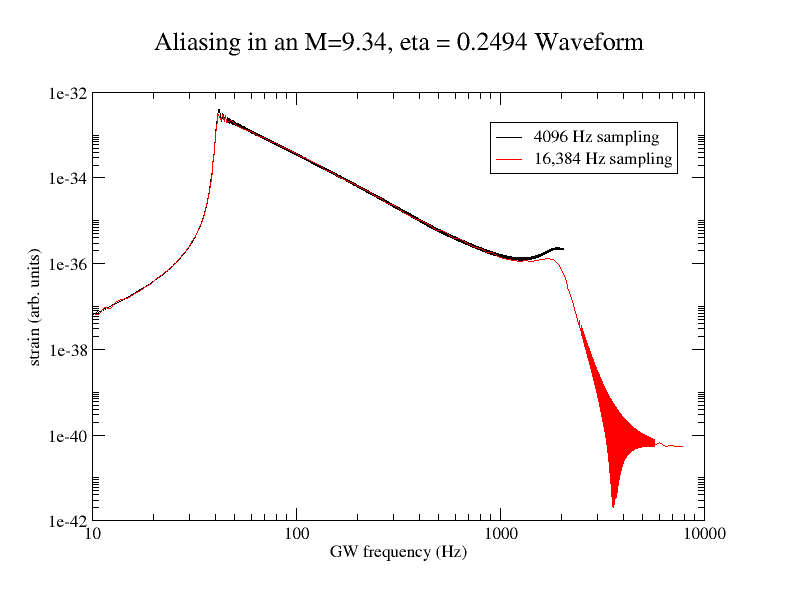
\includegraphics[width=\linewidth]{figures/ninja2_results/ninja2_aliasing}
  \caption[Aliasing of waveform power]{
  \label{f:ninja2_aliasing}
Frequency-domain amplitudes of a NINJA-2 waveform at different
sampling rates.  At a sample rate of 4096 Hz the late portion of the
waveform are distorted due to aliasing of power to lower frequencies.
}
\end{figure}%

Note that this is a different issue from the one that motivated
performing the waveform overlaps at 32768 Hz, discussed in
section~\ref{ssec:ninja2_overlap_comparisons}.  The issue there was
that undersampling could miss the maximum of the overlap function.
The issue here is that undersampling can distort the end of the
waveform.

NINJA-1 consisted of only 127 injections in one day of data, which
severely limited the ability to draw statistical conclusions on the
behavior of the pipelines.  To correct this in NINJA-2 we extended the
duration to eight weeks.  The density of injections was varied over
this span:  weeks 1-3 had one injection on average every 2000 seconds,
week 4-6 had one injection on average every 14,400 seconds, and the
final two weeks had one injection every on average every 216,000
seconds.  The intent is that data analysts can tune and test their
pipelines on the dense weeks, and then optionally perform a
self-blinded test on the final two weeks.

In NINJA-1 the SNR was not chosen a priori but was determined by the
other parameters.  For NINJA-2 we draw the network SNR ($\sqrt{\sum_i
\rho_i^2}$ where $i$ ranges over the IFOs) from a distribution and
then scale the distance of the injection in order to achieve that SNR.
For the first three weeks the distribution is linear from 6 to 130 in
order to allow pipelines to test and tune out to large SNRs on the
densest set of injections.  For the remaining weeks the distribution
falls as the reciprocal of the network SNR (uniform in
$\log(\mathrm{SNR})$) in order to better model the expected
astrophysical distribution.

The mass and waveform selection were also done slightly differently in
NINJA-2.  For each injection a mass was first selected uniformly over
the specified range; for the full 2-month run this range is from
$10-350 \msun$.  Then waveforms were selected at random until one was
found that could be injected at the chosen mass such that the waveform
turns on below 35 Hz.  In practice this condition never caused any
waveform to be rejected, as all submitted waveforms were long enough
to be injected down to the lowest mass in the range.  The mass ratio
and spins are intrinsic to the waveforms, so choosing a submission
amounts to a choice of these parameters as well. 

As in NINJA-1 the sky location and inclination were chosen uniformly
at random.

Four NINJA-2 data sets were released:

\begin{itemize}
\item A test set consisting of one week of data was released on May 13, 2010.  This
included three separate sets spanning different mass regions;
low-mass ($10\msun - 40 \msun$), high-mass ($35 \msun - 100 \msun$)
and a burst/ringdown set ($80 \msun - 350 \msun$).  This purpose of
this run was to shake out bugs in the injection code and waveforms,
several of which were found.

\item A second test set consisting of one week of data for each of the
three mass bins was released on May 31, 2010.  This was meant to test
the fixes implemented after the first test set, and to do more
careful sanity checks.  Some results from this run are discussed in
section~\ref{sec:ninja2_test_week}.

\item Based on positive results from analyses of the second test week,
full two-month data sets for all three mass bins were released on June
9, 2010.  Unfortunately shortly after release a remaining major bug in
the injection software was discovered.  Data is stored in frame files
spanning 4096 seconds.  When an injection crossed frame boundaries
this bug would cause the portion contained in the earlier frame to be
omitted.  This happened in enough cases to invalidate the entire data
set.

\item There was then a lengthy pause, in large part due to the
LIGO-Virgo ``blind injection challenge'' (see
section~\ref{sec:applications_dog}).  However, it was during this time
that the validations discussed in the previous chapter were performed.
It was also in this gap that studies discovered the need to move to
16Hz sampling.   This quadrupled the size of the data and made the
release of 3 separate mass ranges unfeasable.  Therefore a single set
spanning two months and containing injections from $10 \msun - 350
\msun$ was released on June 13, 2011.  Analysis on this set has begun
and some preliminary results will be discussed in
section~\ref{sec:ninjna2_two_months}
\end{itemize}


There are two motivations for constructing and distributing the data
sets as NINJA-1 and NINJA-2 thus far have done.  The first is to
ensure that every group is looking at the same set of injections so
that results can be compared.  The second is due to the terms of the
NINJA agreement, which restricted distribution of the raw NR
waveforms.  However, distribution of such static sets limits the
ability of individual groups to tune their pipelines in optimal ways,
and conceptually distributing a set of parameters would be sufficient
to compare results across pipelines.  In addition the size of the data
sets makes distribution slow and complex.  The NR groups within NINJA
have therefore relaxed the conditions on their use of their waveforms.
Consequently, subsequent NINJA-2 data sets will be distributed as sets
of parameters, and data analysis groups will use the available code to
either create data sets locally, or perform the injections ``on the
fly'' as the analysis is performed.  This will also allow groups to do
special-purpose tuning runs or analyses by injecting specialized 
sets of injections into noise.  The results of these studies may be
published as short-author papers subject to the conditions of the
NINJA agreement.

So far we have focused on simulated Gaussian noise, however as we will
see in the next chapter this is not a good model for the real
detectors.  Real detector data contains many ``glitches'' caused by
both environmental factors and transient behavior of the instruments.
These glitches produce a population of background triggers.  In
testing pipelines a critical issue is the ability to distinguish such
background triggers from signals.  If NINJA is to be able to to make
definitive statements about the behavior of pipelines it is therefore
imperative to use real detector noise.  A memorandum of understanding
has been signed between the NINJA collaboration and the LIGO and Virgo
collaborations allowing the use of real noise from the 5th LIGO and
first Virgo science runs.  There are a number of technical issues to
be resolved before this can be done, however the key results from
NINJA-2 will come from on-the-fly injections into real noise.

\section{CBC Results from the second one-week data set}
\label{sec:ninja2_test_week}

As noted above, two one-week data sets were produced for testing the
injection code and performing sanity checks on the results.  Here we
present the results of running the standard low-mass CBC pipeline on
the low-mass data set from the second of these runs.  As this was
largely a testing and debugging exercise no effort was made to draw
conclusions about the pipelines.  In particular, no runs were
performed with a bank extended to unphysical $\eta$ or the other
pipeline modifications suggested by the studies in
chapter~\ref{ch:comparison} and tested in NINJA-1.

The injection parameters were chosen as described above, the selected
masses, spins and distances are shown in
figure~\ref{f:ninja2_test_dataset}.

\begin{figure}
  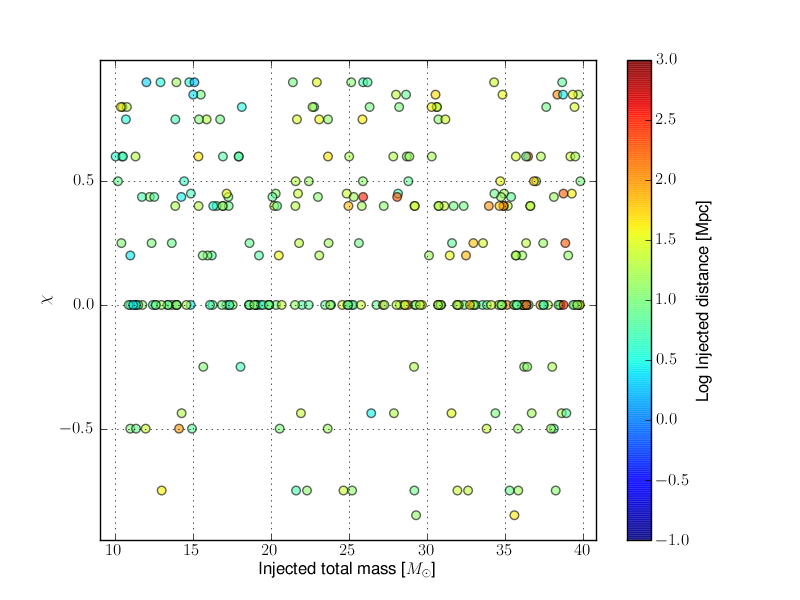
\includegraphics[width=\linewidth]{figures/ninja2_results/ninja2_test_dataset.png}
  \caption[Parameters of the NINJA-2 test one-week data set]{
  \label{f:ninja2_test_dataset}
Distribution of mass, spin and distance parameters in the one-week,
Gaussian-noise test data set.
}
\end{figure}%


The S6 version of the standard CBC low-mass pipeline was run over this
data set.  This version of the pipeline uses Taylor F2
stationary-phase templates taken to 3.5 pN order in phase evolution.
The first result of interest is the found/missed plots at the first
stage, before the $\chisq$ test or coincidence between detectors has
been applied.  The result for the H1 detector is shown in
figure~\ref{f:first_stage}.  This can give some indication of how well
the waveforms and the bank capture the signals.  However, it can also
be misleading.  The pipeline considers an injection to be ``found'' if
there is a trigger within 100 ms of the injection time.  No parameter
matching is required.  This means a quiet trigger resulting from the
noise can be mistaken for finding the injection.  To see how often
this can happen we also ran the analysis on frames containing only the
noise, without any injected signals.  This is also shown in
figure~\ref{f:first_stage}, and indeed many of the reportedly-found
injections can be seen to be coming from the noise.  Both $\chisq$ and
coincidence will cut down the number of false reports, in
figure~\ref{f:test_found_missed} we show the found/missed plots for
all three detectors after the coincidence test, and many of the
triggers coming from the background have been removed.  At the second
stage the results are sensible, the ability of the pipeline to recover
the injections falls off as the effective distance increases.  There
are however a few close missed injections that would warrant follow up
study in a full search.


\begin{figure}
  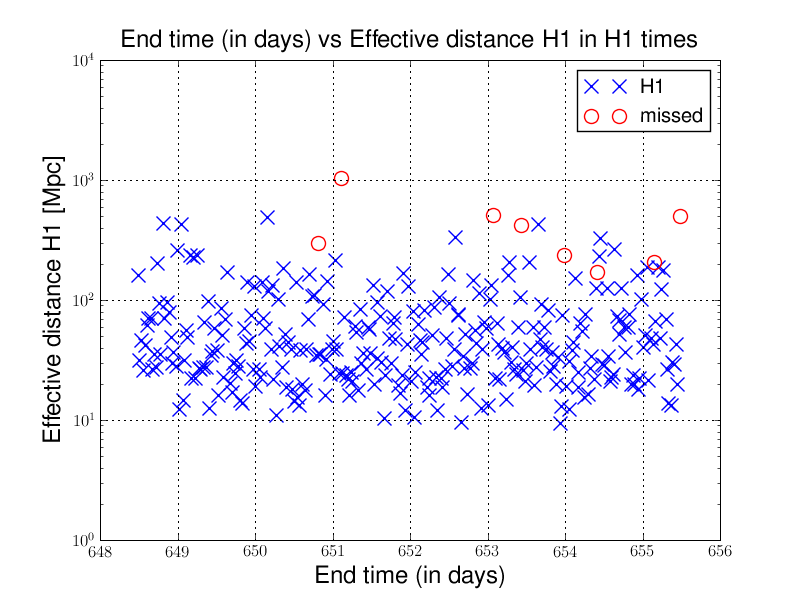
\includegraphics[width=0.5\linewidth]{figures/ninja2_results/h1-plotinspmissed_full_data_time-eff_dist-log-h1-871147524-606064.png}
  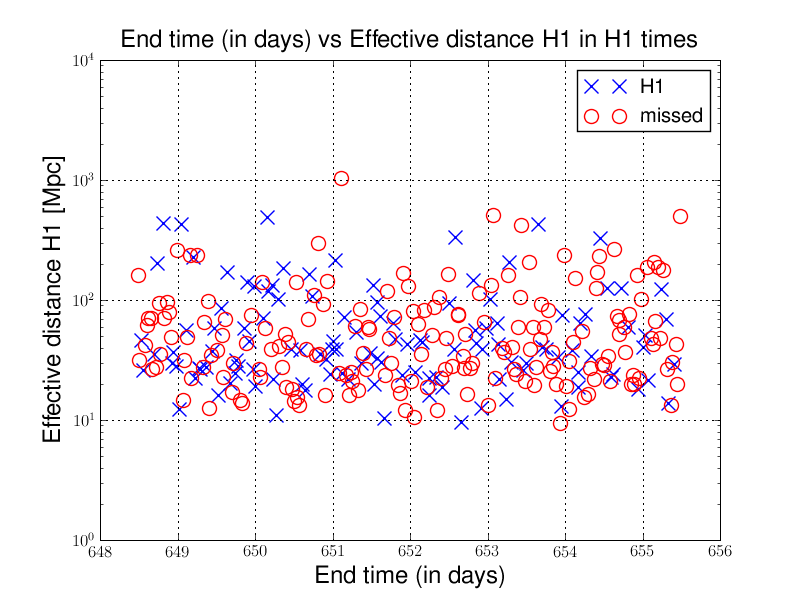
\includegraphics[width=0.5\linewidth]{figures/ninja2_results/h1-plotinspmissed_full_data_time-eff_dist-log-h1-871147524-606064_noiseonly.png} \\
  \caption[First-stage found/missed from the test data set]{
  \label{f:first_stage}
First-stage found/missed plots from the test data set.  On the left,
the results from the data set containing the injections, on the right
the results from running on the noise-only data.  Many signals appear
in both, indicating that they are not really found, but only that
there is a random background trigger within the time window.
}
\end{figure}%



\begin{figure}
  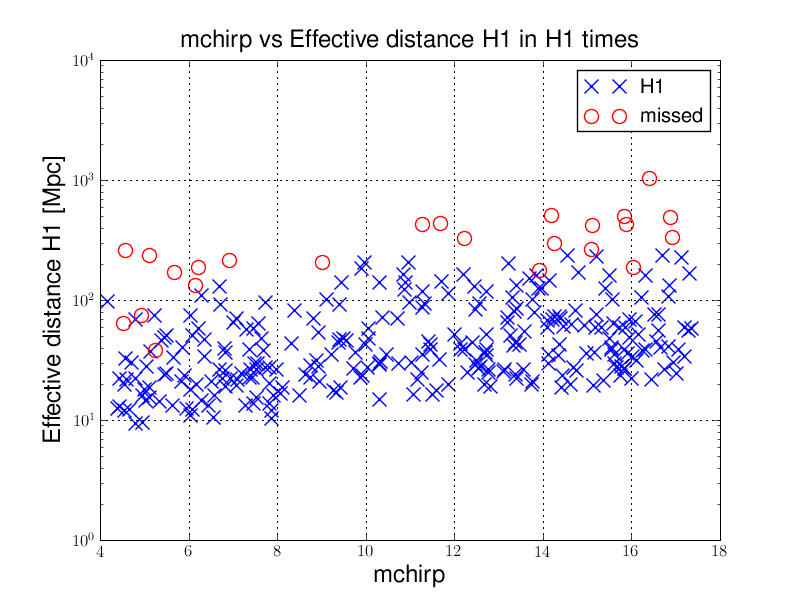
\includegraphics[width=0.5\linewidth]{figures/ninja2_results/h1-plotinspmissed_full_data_mchirp-eff_dist-log-h1-871147524-606064_second}
  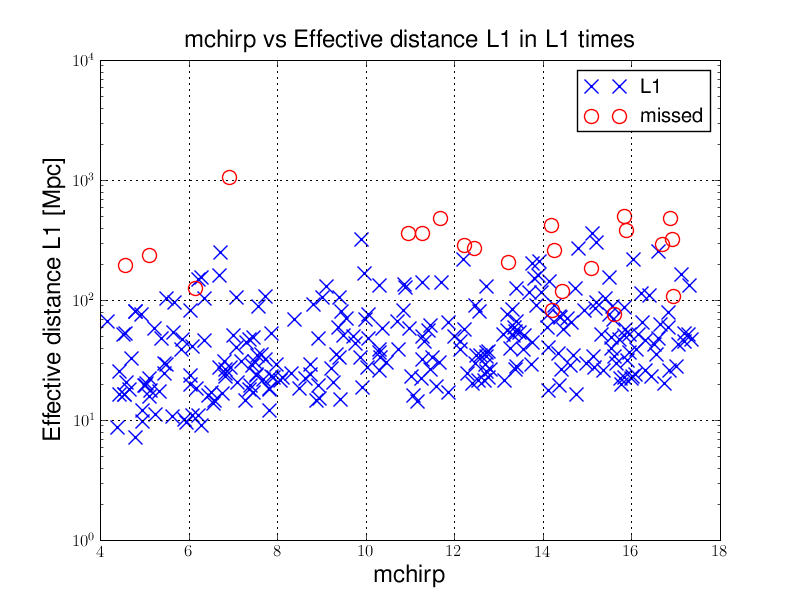
\includegraphics[width=0.5\linewidth]{figures/ninja2_results/l1-plotinspmissed_full_data_mchirp-eff_dist-log-l1-871147524-606064_second} \\
  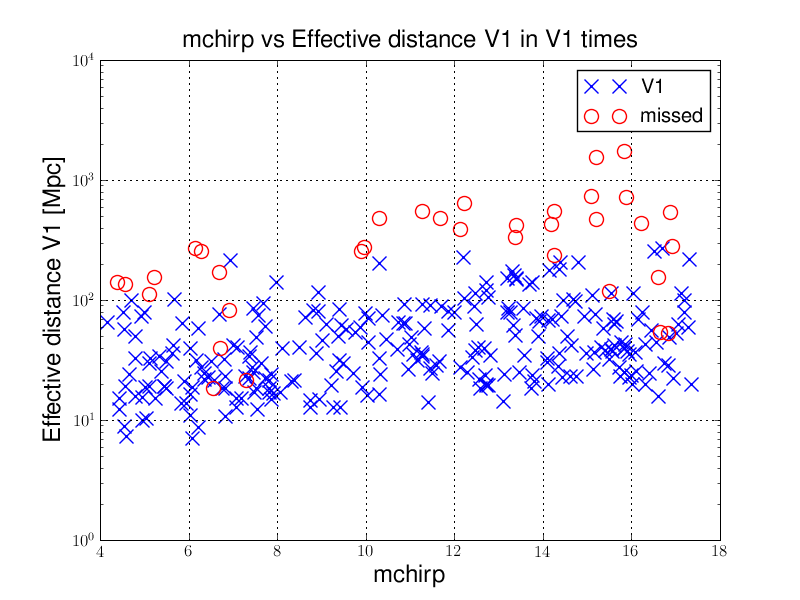
\includegraphics[width=0.5\linewidth]{figures/ninja2_results/v1-plotinspmissed_full_data_mchirp-eff_dist-log-v1-871147524-606064_second}
  \caption[Second-stage found-missed plots for the test data set]{
  \label{f:test_found_missed}
Second-stage found/missed plots for the test data set, for all three
detectors.  Each plot shows signals that were reovered in that
detector and at least one other.  Requiring coincidence removes the
background triggers seen in figure~\ref{f:first_stage}.  The results
are sensible: closer injections are more likely to be found than
distant ones.
}
\end{figure}%


In figure~\ref{f:test_recovered_snr} we plot the SNR recovered by the
pipeline versus the injected value.  There is a distinct pattern
exhibited, for low-mass signals the injected and recovered SNR match,
but the recovered SNR drops off with increasing mass.  This occurs
because the injected SNR value is calculated using the entire
waveform.  By contrast the recovered value terminates the integration
at the ISCO frequency.  For higher-mass systems this means the
integration cuts off in or before the sensitive band, while there is
still power in the signal, and consequently the SNR is underestimated.
While we can not hope to capture the full merger and ringdown with
inspiral-only templates, this again confirms the results of
chapter~\ref{ch:comparison} and NINJA-1, which show that extending the
templates to high frequencies can increase the SNR.

\begin{figure}
  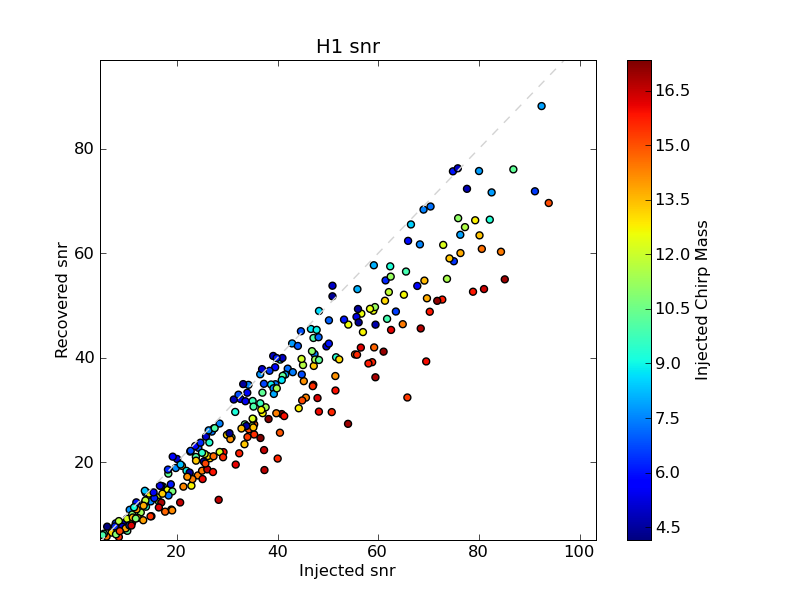
\includegraphics[width=0.5\linewidth]{figures/ninja2_results/h1_snrs_second}
  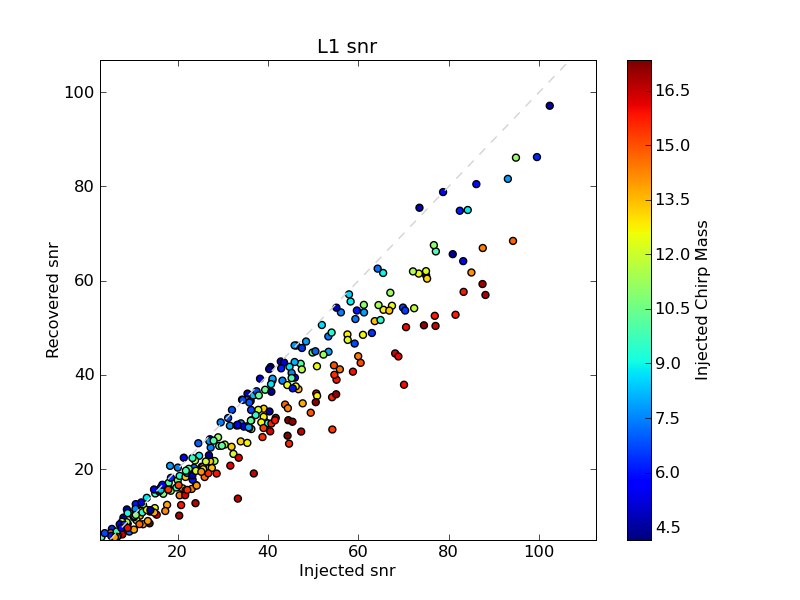
\includegraphics[width=0.5\linewidth]{figures/ninja2_results/l1_snrs_second} \\
  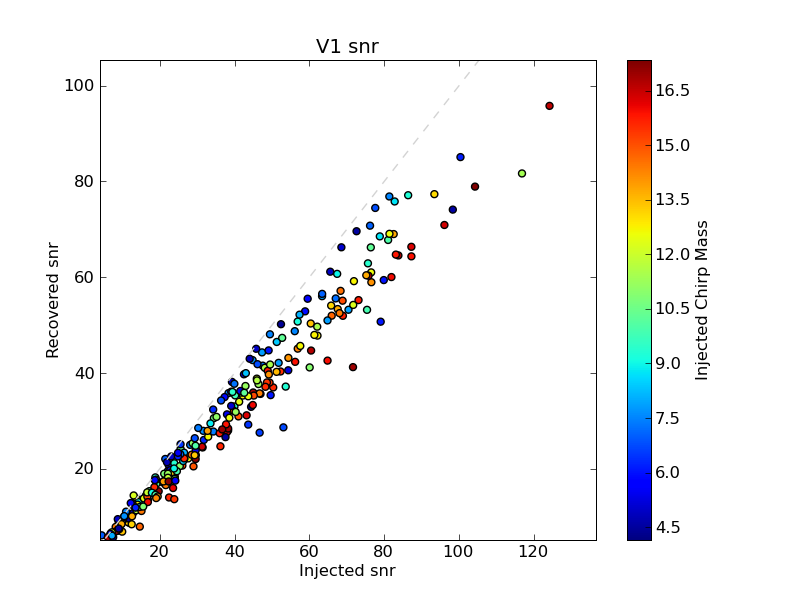
\includegraphics[width=0.5\linewidth]{figures/ninja2_results/v1_snrs_second}
  \caption[SNR recovery for the test data set]{
  \label{f:test_recovered_snr}
SNR recovery for the test data set in all three detectors.  The
injected SNR is calculated from the entire waveform, the recovered SNR
is calculated only from the inspiral up to the ISCO frequency.  At
higher masses this loses SNR as the late inspiral, merger, and
ringdown pass through the detector sensitive bands.  Note that V1,
which has lower noise at low frequencies, recovers somewhat more SNR
for the high-mass systems.
}
\end{figure}%


\iffalse
Can add if desired.
\begin{figure}
  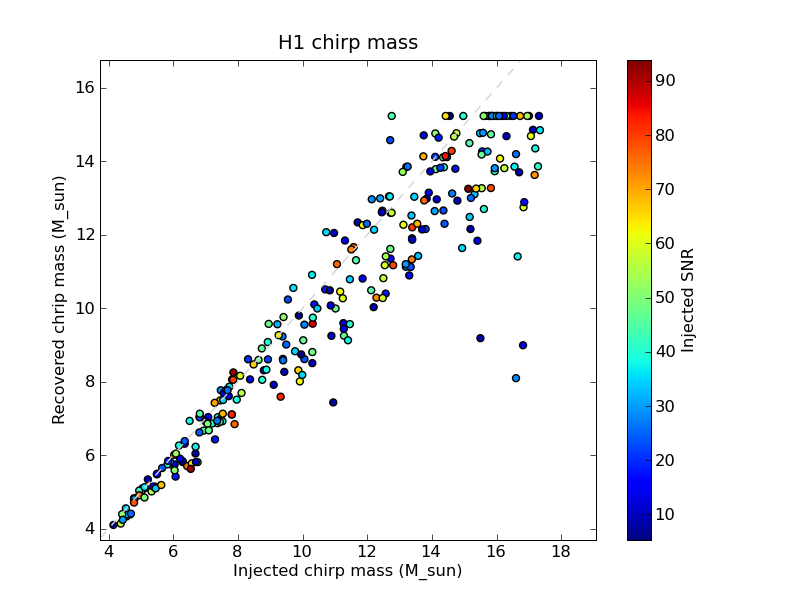
\includegraphics[width=0.5\linewidth]{figures/ninja2_results/h1_masses_second}
  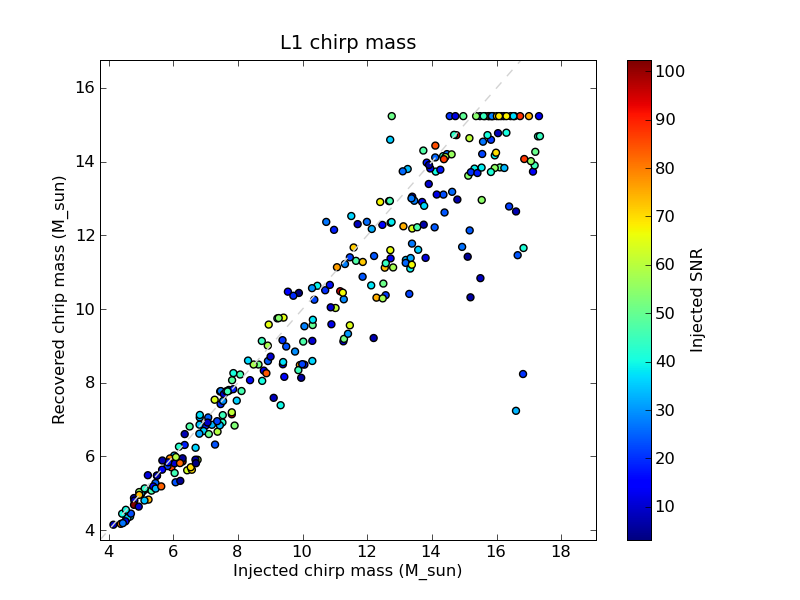
\includegraphics[width=0.5\linewidth]{figures/ninja2_results/l1_masses_second} \\
  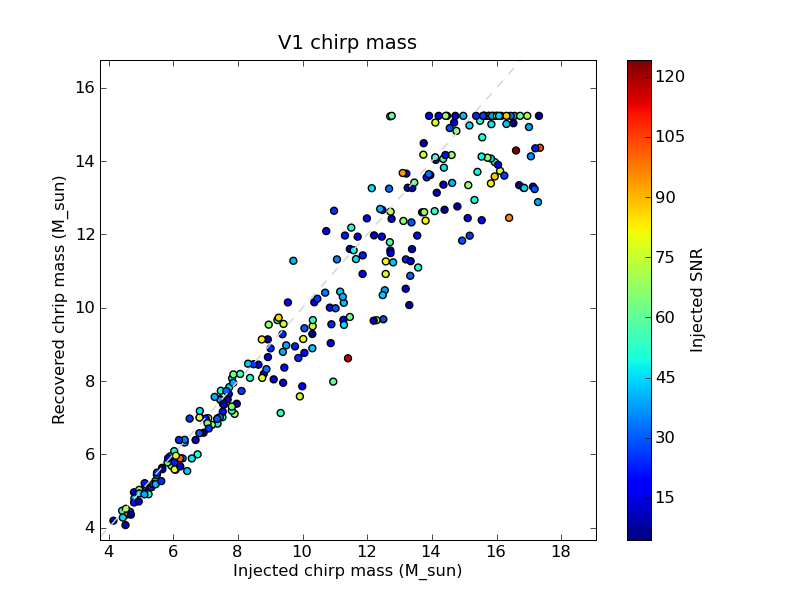
\includegraphics[width=0.5\linewidth]{figures/ninja2_results/v1_masses_second}
  \caption[Mass recovery for the test data set]{
  \label{f:test_recovered_snr}
}
\end{figure}%
\fi

At the level of investigation performed the results from this data set
appear reasonable.  Although conversely this means that the waveform
truncation issue discussed above was not caught by this investigation.
However, this and other analyses did indicate that there were no other
more serious bugs in the injection software, which enabled us to move
to the full two-month set.

\section{CBC Results from the two-month data set}
\label{sec:ninjna2_two_months}

We now turn to the second two-month data set in Gaussian noise.  This
is the latest set constructed, and includes many corrections and
changes from earlier sets:

\begin{itemize}
\item The data is now sampled at 16,384 Hz.
\item There is now only one set spanning the full mass range from $10
\msun - 350 \msun$.
\item The waveforms have been updated, in particular many of the
hybridizations were redone.
\end{itemize}


Apart from the change in mass range the injection parameters were
chosen as described above.  The masses, spins, and distances chosen
are shown in figure~\ref{f:ninja2_dataset}.

\begin{figure}
  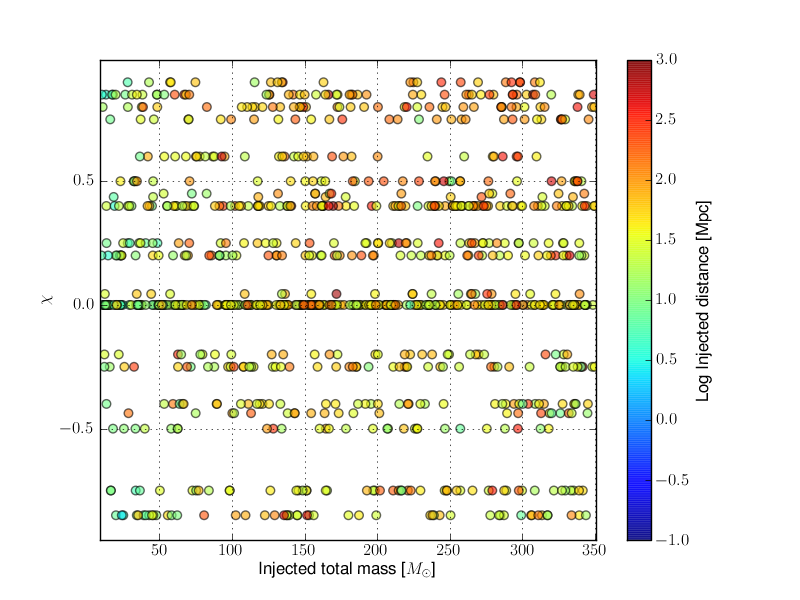
\includegraphics[width=\linewidth]{figures/ninja2_results/ninja2_dataset}
  \caption[Parameters of the NINJA-2 two-month data set]{
  \label{f:ninja2_dataset}
Distribution of mass, spin and distance parameters in the two-month,
Gaussian-noise data set.
}
\end{figure}%


\iffalse
Real detector data is far from Gaussian, and real data analysis is
concerned not only with foreground triggers from signals but also
background triggers from noise.  In order to comprehensively test the
ability of pipelines to detect signals and recover their parameters it
is necessary to perform injections into real detector noise.  As of
this writing a memorandum of understanding (MoU) between the NINJA
collaboration, the LIGO collaboration and the Virgo collaboration has
been signed which will allow subsequent NINJA-2 data sets to use data
from the previous (S5/VSR1) science run as noise.  A key feature of
this agreement is that NINJA is not a gravitational wave search.  We
will therefore use data from disjoint periods in each instrument.
Details of this plan, such as which times to use, have yet to be
decided.  However it is clear we will need a custom segment database
(see chapter~\ref{ch:detchar}) to mark times where the instruments
were glitching. However, injection times will not use this
information, as it is entirely possible that real signals will land on
or near a glitch, and the ability to detect such signals is an
important test.
\fi


This data set was analyzed with the standard CBC low-mass and
high-mass pipelines.  The parameters were exactly as in the S6/VSR2,3
runs, no changes were made to the configurations except for those
relating to the names of the data files.  The low-mass search uses
Taylor F2 templates to 3.5 pN order in phase evolution
(section~\ref{sec:PNWaveforms}) in a mass region defined by minimum
component masses of $1 \msun$ and maximum total mass of $25 \msun$.
The high mass search uses EOBNR templates (section~\ref{ssec:EOB}) in
a region defined by minimum component masses of $1 \msun$, minimum
total mass of $25 \msun$, and maximum total mass of $100 \msun$.


Figure~\ref{f:ninja2_cbc_results_high_first} shows the found/missed plots
after the first stage in the high-mass search.  As expected, distant
signals are less likely to be found than close ones.  As discussed
above the loose coincidence test between injections and triggers means
that many of these injections may not really be found.  We therefore
look at the second-stage results in
figure~\ref{f:ninja2_cbc_results_high_second}, and as in
figure~\ref{f:first_stage} there are many fewer found injections.  


\begin{figure}
  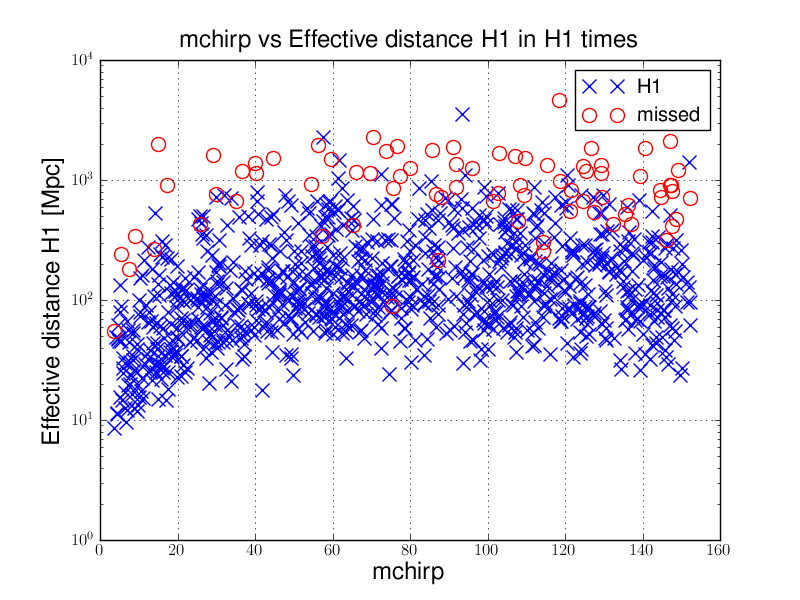
\includegraphics[width=0.5\linewidth]{figures/ninja2_results/H1-plotinspmissed_HIGH_FULL_DATA_mchirp-eff_dist-log-H1-871147552-5209912_first} 
  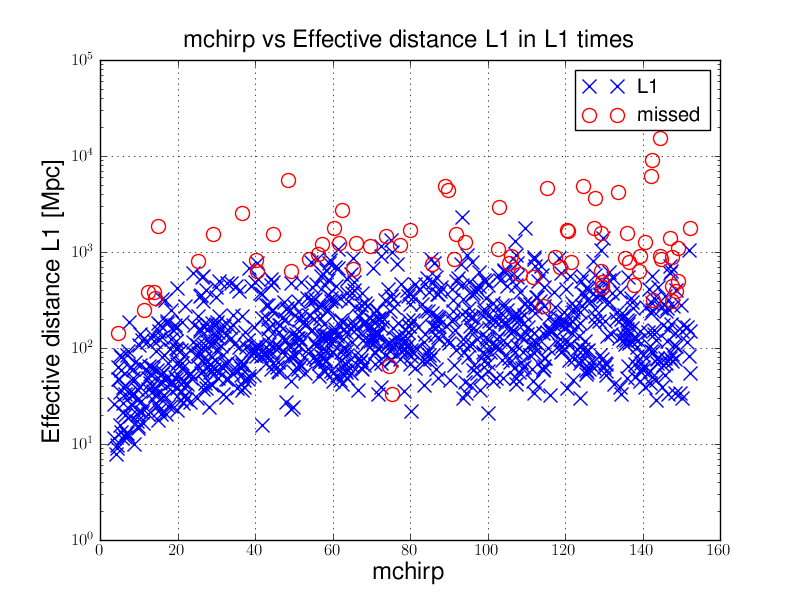
\includegraphics[width=0.5\linewidth]{figures/ninja2_results/L1-plotinspmissed_HIGH_FULL_DATA_mchirp-eff_dist-log-L1-871147552-5209912_first} \\
  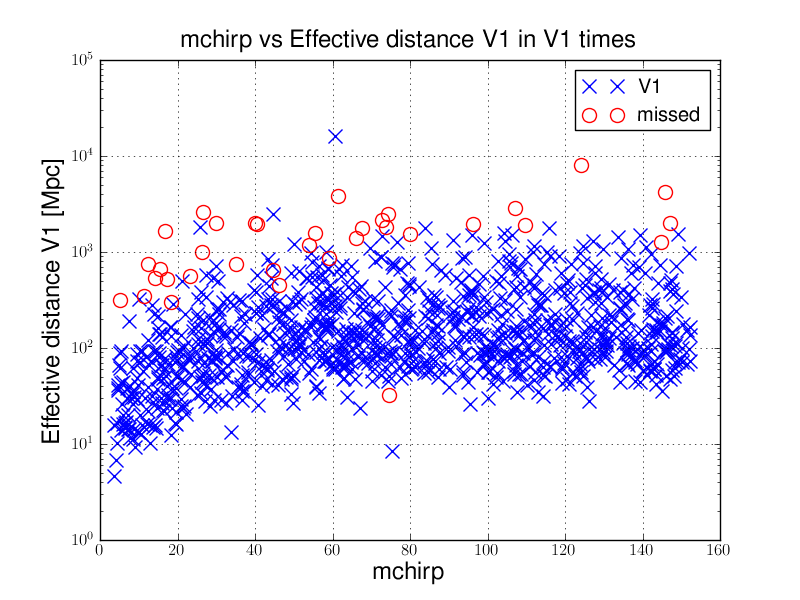
\includegraphics[width=0.5\linewidth]{figures/ninja2_results/V1-plotinspmissed_HIGH_FULL_DATA_mchirp-eff_dist-log-V1-871147552-5209912_first} \\
  \caption[First stage found/missed plots from the high-mass search]{
  \label{f:ninja2_cbc_results_high_first}
Preliminary first stage found/missed plots from the high-mass search.
The behavior is as expected: distant signals are more likely to be
missed than close ones.
}
\end{figure}%

\begin{figure}
  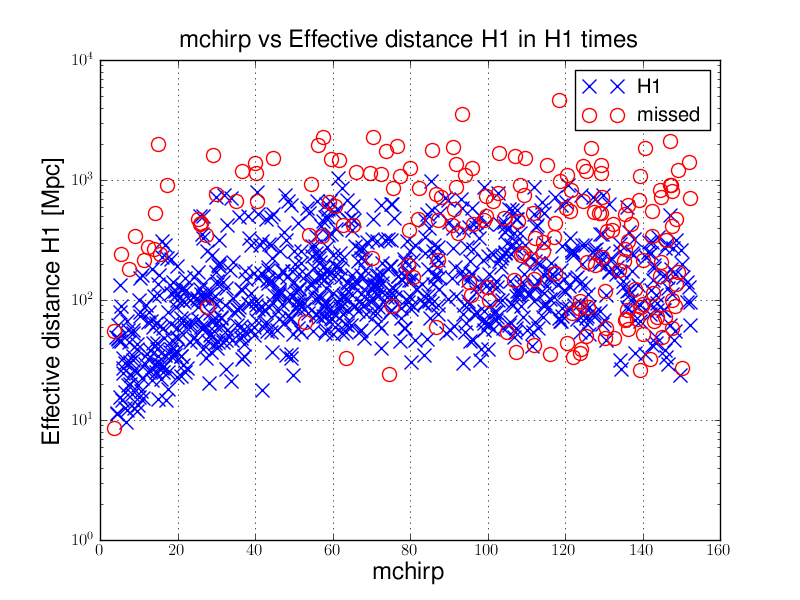
\includegraphics[width=0.5\linewidth]{figures/ninja2_results/H1-plotinspmissed_HIGH_FULL_DATA_mchirp-eff_dist-log-H1-871147552-5209912} 
  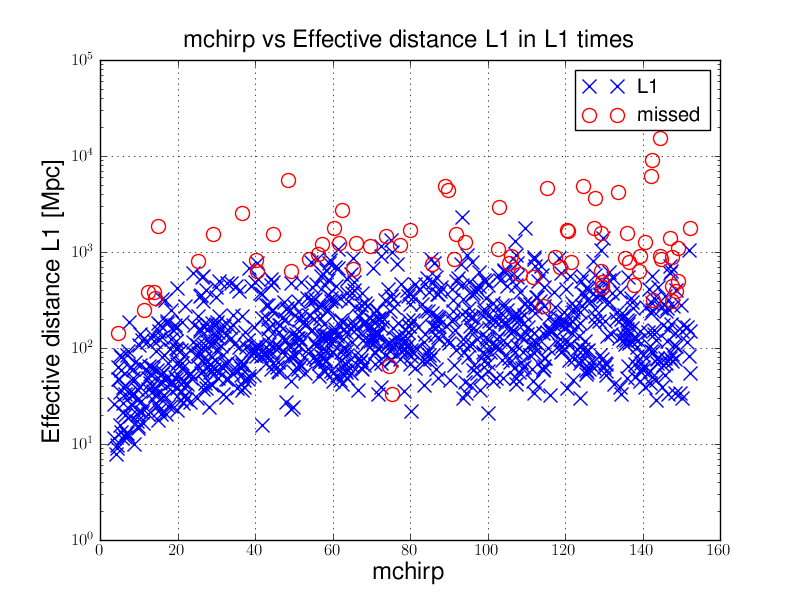
\includegraphics[width=0.5\linewidth]{figures/ninja2_results/L1-plotinspmissed_HIGH_FULL_DATA_mchirp-eff_dist-log-L1-871147552-5209912} \\
  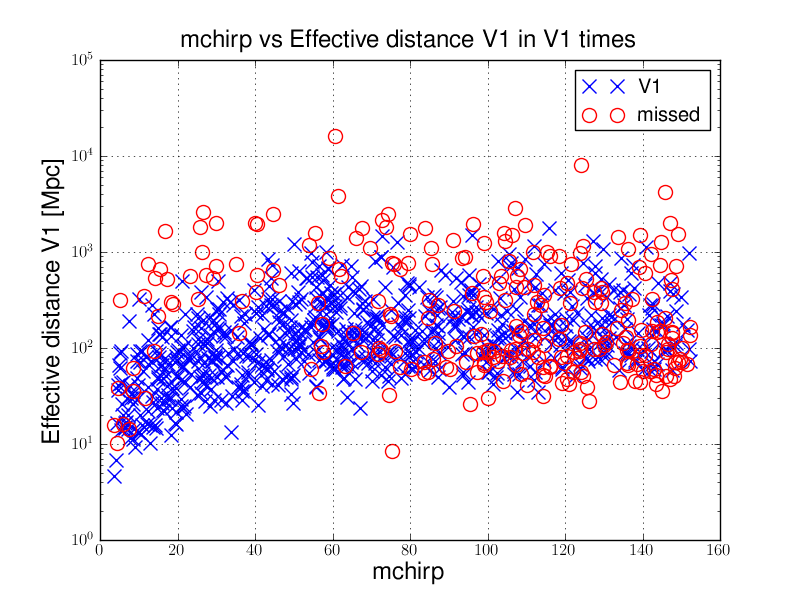
\includegraphics[width=0.5\linewidth]{figures/ninja2_results/V1-plotinspmissed_HIGH_FULL_DATA_mchirp-eff_dist-log-V1-871147552-5209912} \\
  \caption[Second stage found/missed plots from the high-mass search]{
  \label{f:ninja2_cbc_results_high_second}
Preliminary second stage (after coincidence and $\chisq$) found/missed plots from
the high-mass search.  As expected, many of the signals reported as
``found'' after the first stage were due to background triggers within
100 ms of the injection.  More signals are missed at higher masses
because the high-mass bank only extends to $100 \msun$ but there are
injections up to $350 \msun$.  There is an anomaly in the Virgo
results, see the text for discussion.
}
\end{figure}%

The fraction of injections found decreases with increasing mass.  The
bank of the high-mass search extends only to $100 \msun$, but the
injections extend up to $350 \msun$, so this result is not surprising.
We can quantify the effect by plotting the efficiency, defined as this
fraction, as a function of mass.  These plots are shown in
figure~\ref{f:high_mass_efficiencies}.  While these plots show the
general trend, they are quite jagged, indicating that we do not have
enough injections to draw statistical conclusions.  Follow up work
will remedy this by performing many thousands of ``on the fly''
injections.

There is an unexpected feature in the V1 plot, which shows that at
high mass more close injections are missed than distant ones.  We
will return to this issue below.


\begin{figure}
  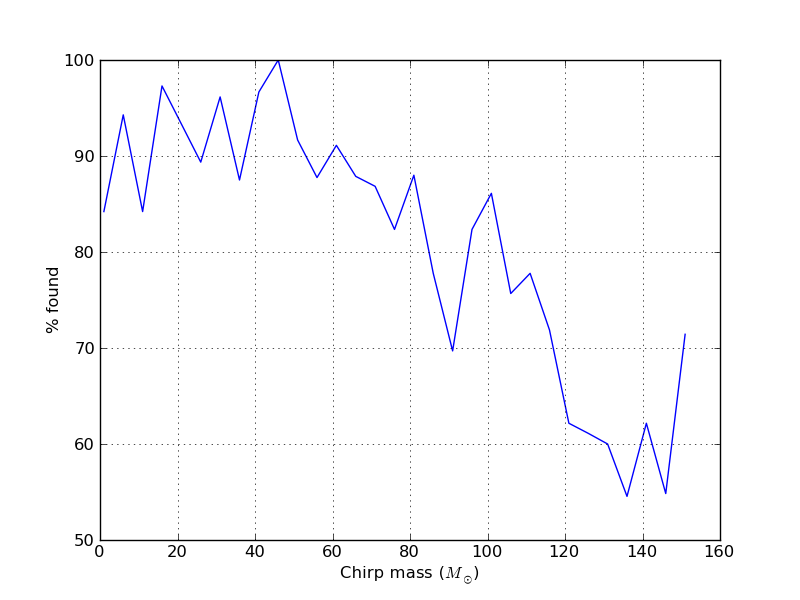
\includegraphics[width=0.5\linewidth]{figures/ninja2_results/H_second_mass_high_efficiency}
  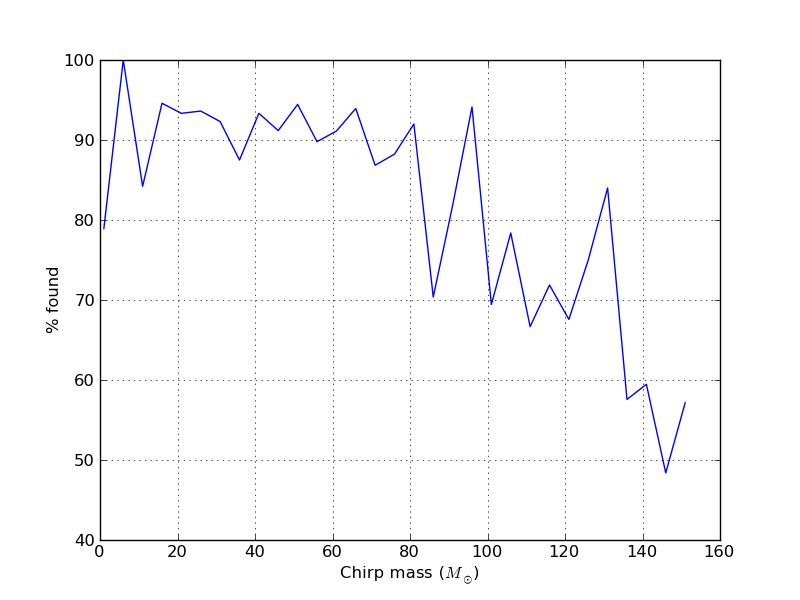
\includegraphics[width=0.5\linewidth]{figures/ninja2_results/L_second_mass_high_efficiency} \\
  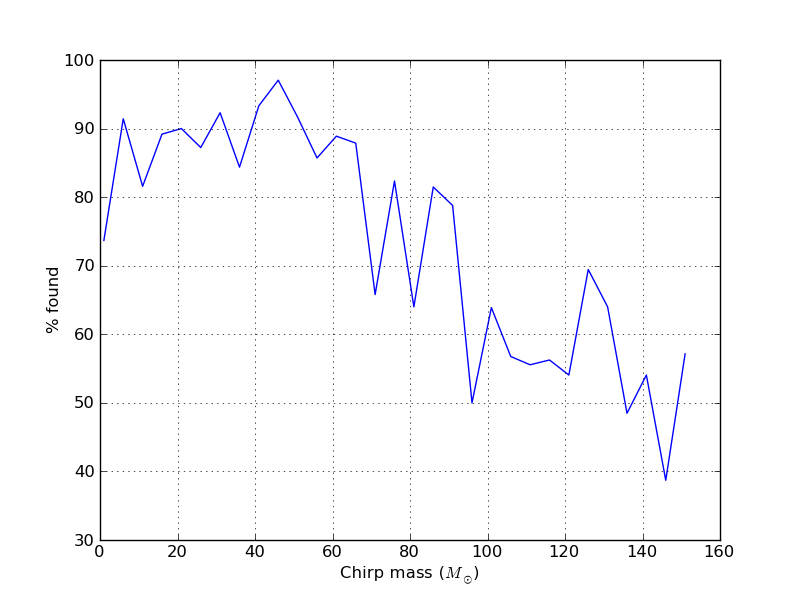
\includegraphics[width=0.5\linewidth]{figures/ninja2_results/V_second_mass_high_efficiency}
  \caption[Efficiency of the high-mass pipeline as a function of mass]{
  \label{f:high_mass_efficiencies}
Efficiencies of the high-mass pipeline as a function of mass.  As
can be seen in figure ~\ref{f:ninja2_cbc_results_high_second} the
efficiencies decrease as mass increases.  However, the jaggedness in
these plots indicates that there are not enough injections to draw
definitive conclusions.
}
\end{figure}%

The standard CBC low-mass and high-mass searches both use non-spinning
templates, and an important question is the ability of these pipelines
to detect spinning signals.  NINJA-2 is uniquely positioned to help
answer this question, and we begin by plotting the recovery efficiency
of the high-mass pipeline as a function of the spin parameter $\chi$
in figure~\ref{f:high_spin_efficiencies}.  There is a general trend
suggesting that the efficiency increases with $\chi$, and in
particular that the search performs worse on anti-aligned systems than
aligned systems.  Again, the jaggedness of the plots makes it
impossible to draw definitive conclusions, this will be remedied in
follow up studies with more injections.



\begin{figure}
  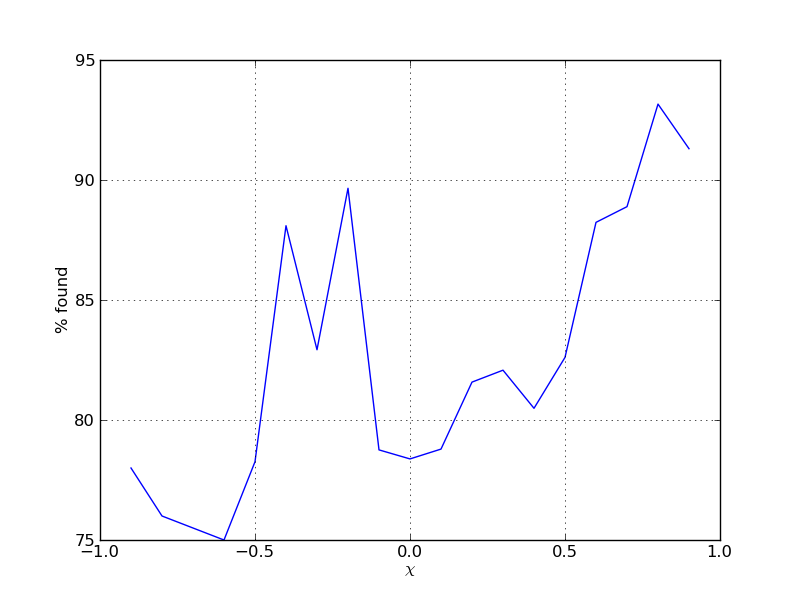
\includegraphics[width=0.5\linewidth]{figures/ninja2_results/H_second_spin_high_efficiency}
  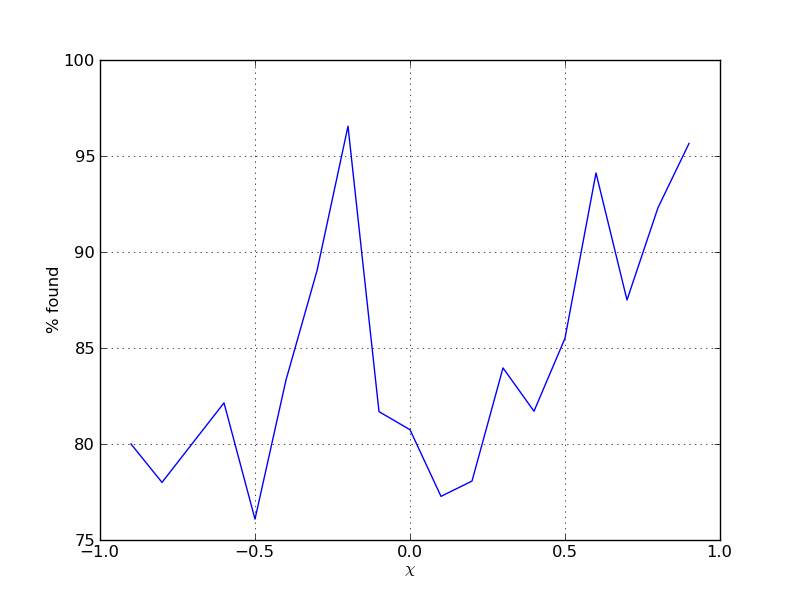
\includegraphics[width=0.5\linewidth]{figures/ninja2_results/L_second_spin_high_efficiency} \\
  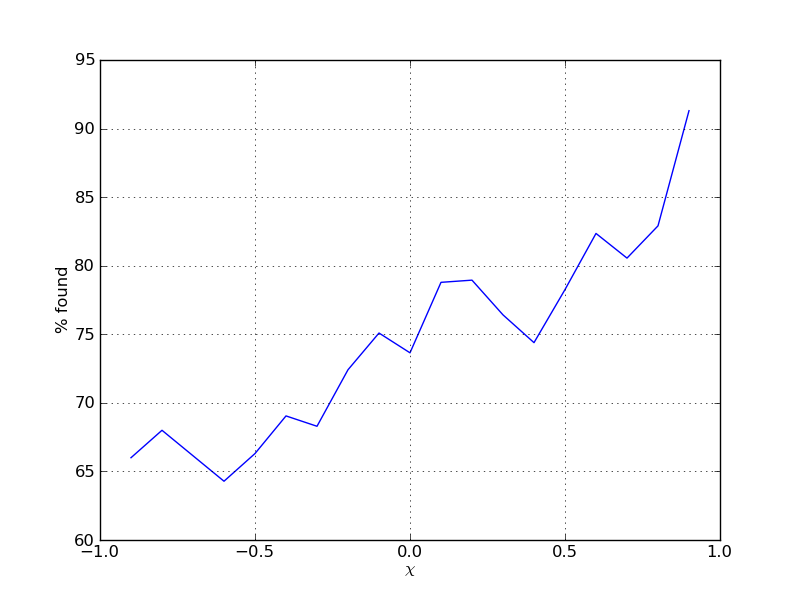
\includegraphics[width=0.5\linewidth]{figures/ninja2_results/V_second_spin_high_efficiency}
  \caption[Efficiency of the high-mass pipeline as a function of mass]{
  \label{f:high_spin_efficiencies}
Efficiencies of the high-mass pipeline as a function of the spin
parameter $\chi$.  There is a general trend suggesting the pipeline
is more efficient at detecting aligned spins, but more injections are
needed to verify and quantify this.
}
\end{figure}%


We now consider the parallel analysis performed with the low-mass
search.  Figure~\ref{f:ninja2_cbc_results_low_first} shows the
found/missed plots after the first stage.  Again, distant signals are
more likely to be missed than close ones.  The low-mass template bank
extends to a total mass of $25\msun$, and correspondingly the
efficiency decreases notably above a chirp mass of $\approx 80 \msun$.

The anomalous behavior in Virgo is more pronounced here than in the
high-mass search, with most injections above a chirp mass of $100
\msun$ and closer than $100$ Mpc being missed.  We return to this
issue in section~\ref{ssec:virgo_anomaly}.

Figure~\ref{f:ninja2_cbc_results_low_second} shows the found/missed
plots after the second stage.  Again, many of the injections reported
as found in the first stage are now reported as missed.  The remaining
found injections are clustered towards the low end of the mass range,
as expected.  However, in all IFOs at this stage the remaining found
injections at higher masses tend to be at farther distances, contrary
to the expected behavior.  In addition, the injections found in V1 are
mostly confined to the region $M_{chirp} < 20 \msun$, whereas those in
H1 and L1 extend up to $\approx 60 \msun$.  This indicates that most
of triggers above $20 \msun$ are found in coincidence between H1 and
L1.  In turn this implies that signals above this point are either not
really found in V1 at the first stage, or are seen with very different 
parameters that fail the coincident test with the H1 and L1 triggers.
Again we defer further discussion to section~\ref{ssec:virgo_anomaly}.


\begin{figure}
  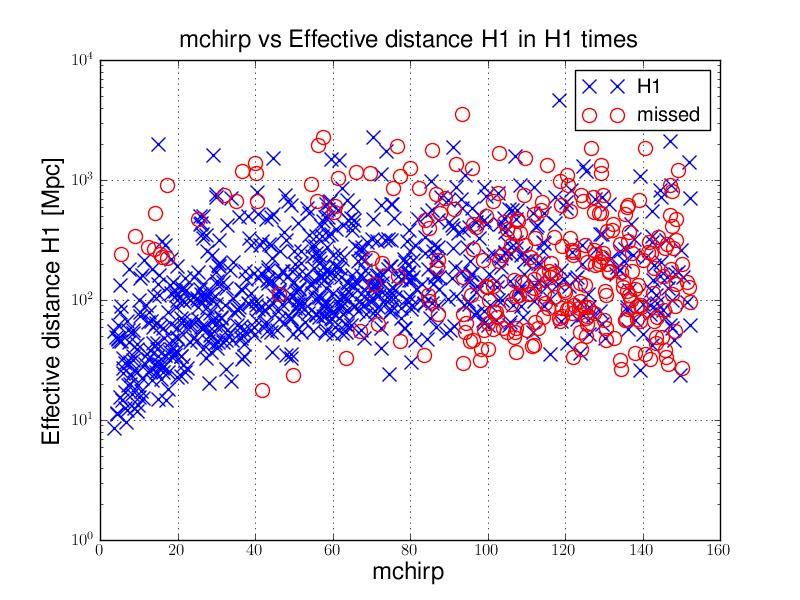
\includegraphics[width=0.5\linewidth]{figures/ninja2_results/H1-plotinspmissed_LOW_FULL_DATA_mchirp-eff_dist-log-H1-871147552-5209912_first} 
  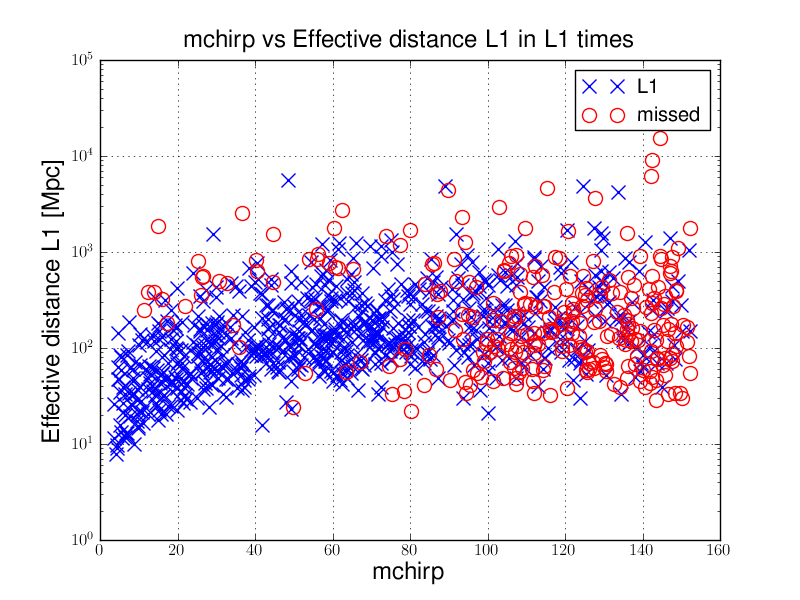
\includegraphics[width=0.5\linewidth]{figures/ninja2_results/L1-plotinspmissed_LOW_FULL_DATA_mchirp-eff_dist-log-L1-871147552-5209912_first} \\
  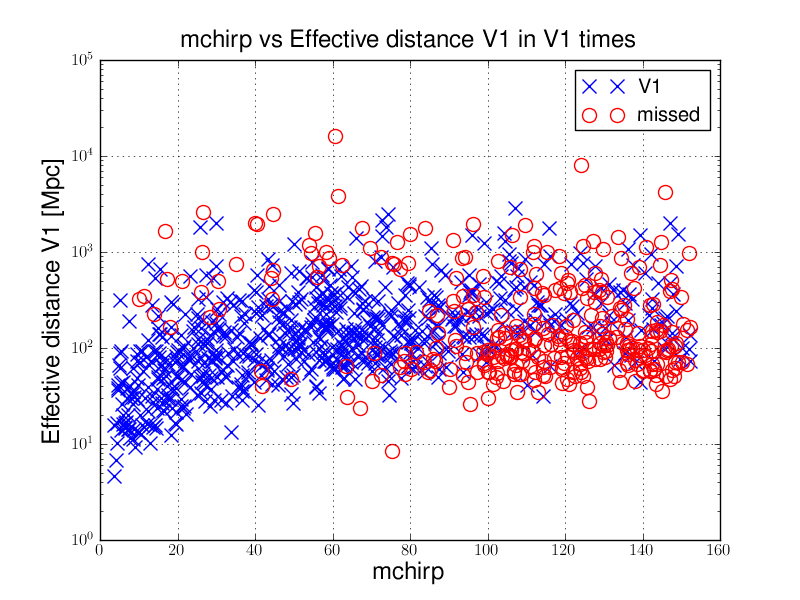
\includegraphics[width=0.5\linewidth]{figures/ninja2_results/V1-plotinspmissed_LOW_FULL_DATA_mchirp-eff_dist-log-V1-871147552-5209912_first} \\
  \caption[First stage found/missed plots from the low-mass search]{
  \label{f:ninja2_cbc_results_low_first}
Preliminary first stage found/missed plots from the low-mass search.
The behavior is as expected: distant signals are more likely to be
missed than close ones.
}
\end{figure}%

\begin{figure}
  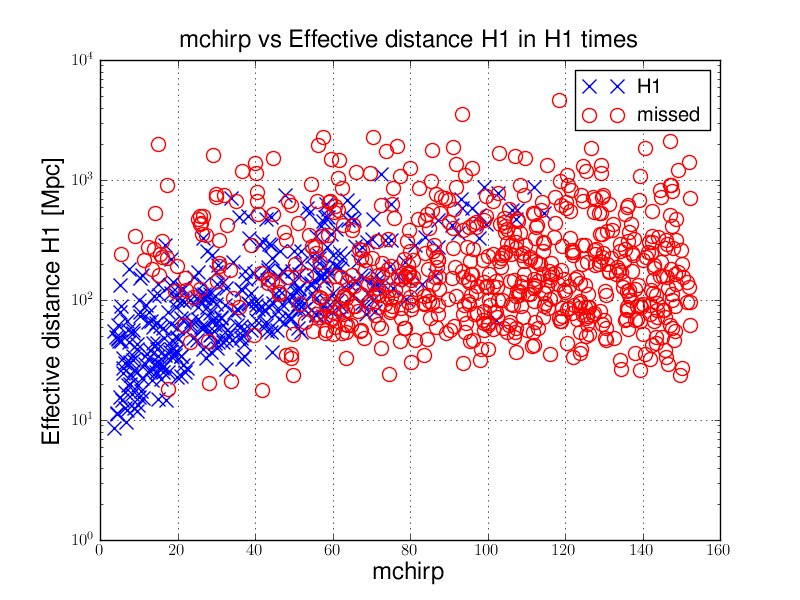
\includegraphics[width=0.5\linewidth]{figures/ninja2_results/H1-plotinspmissed_LOW_FULL_DATA_mchirp-eff_dist-log-H1-871147552-5209912} 
  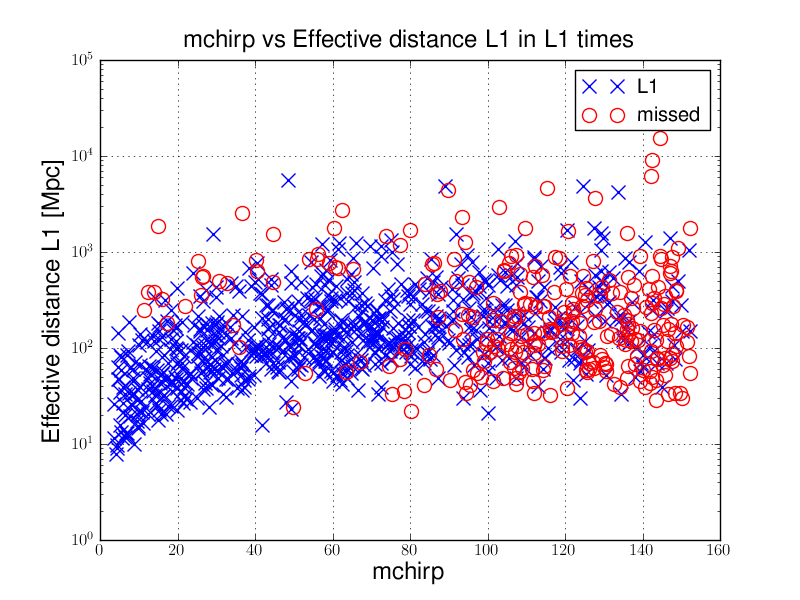
\includegraphics[width=0.5\linewidth]{figures/ninja2_results/L1-plotinspmissed_LOW_FULL_DATA_mchirp-eff_dist-log-L1-871147552-5209912} \\
  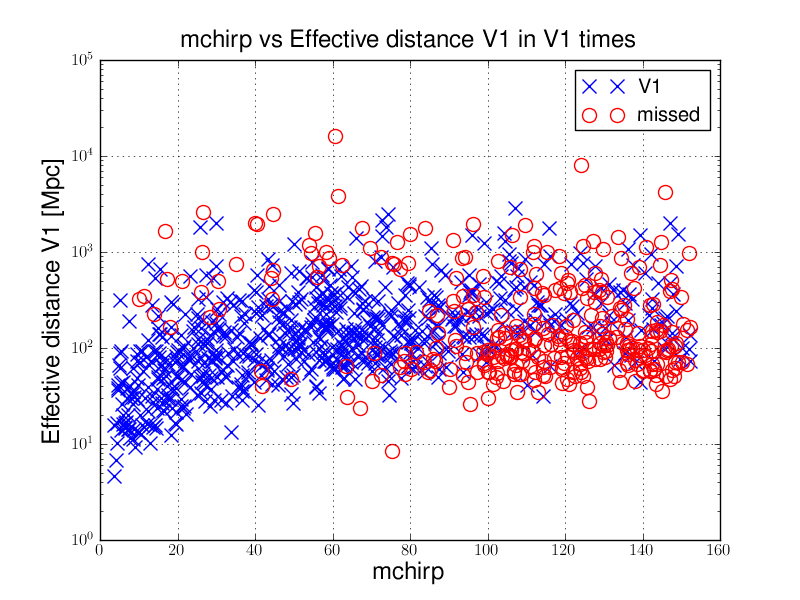
\includegraphics[width=0.5\linewidth]{figures/ninja2_results/V1-plotinspmissed_LOW_FULL_DATA_mchirp-eff_dist-log-V1-871147552-5209912} \\
  \caption[Second stage found/missed plots from the low-mass search]{
  \label{f:ninja2_cbc_results_low_second}
Preliminary second stage found/missed plots from
the low-mass search.  Virgo appears to only find injections below a
chirp mass of $20 \msun$, all found injections above this point come
from coincidences between H1 and L1.  In all IFOs injections found at
higher masses have larger effective distances.  Further studies are
needed to understand this behavior, see
section~\ref{ssec:virgo_anomaly}.
}
\end{figure}%

The efficiencies of the pipeline as a function of mass is shown in
figure~\ref{f:low_mass_efficiencies}, and as a function of spin in
figure~\ref{f:low_spin_efficiencies}.  The mass plots present the
same information found in figure~\ref{f:ninja2_cbc_results_low_second}
in an alternate way, and as in the corresponding high-mass plots
indicate that more injections are needed in order to refine the
results.  The spin plots show the same general trend in the high-mass
plots, again indicating that the search is more efficient at detecting
systems with aligned spins than anti-aligned.

\begin{figure}
  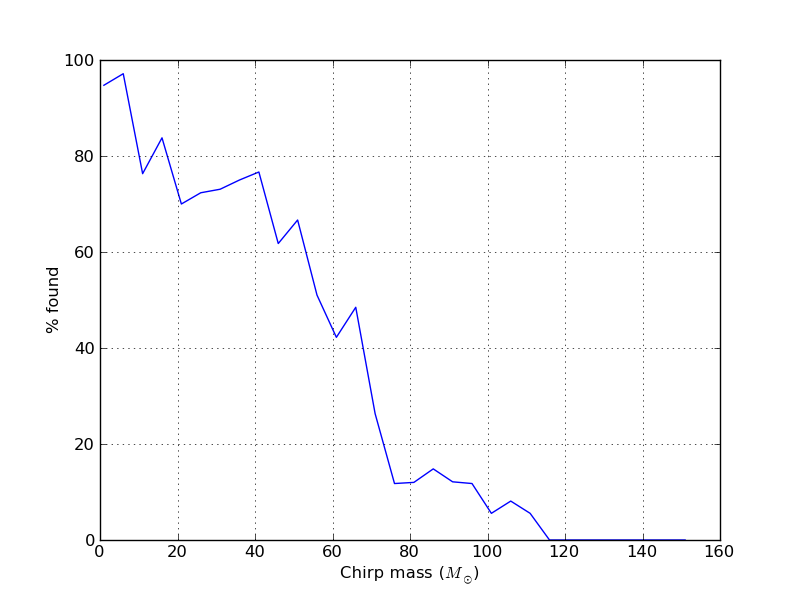
\includegraphics[width=0.5\linewidth]{figures/ninja2_results/H_second_mass_low_efficiency}
  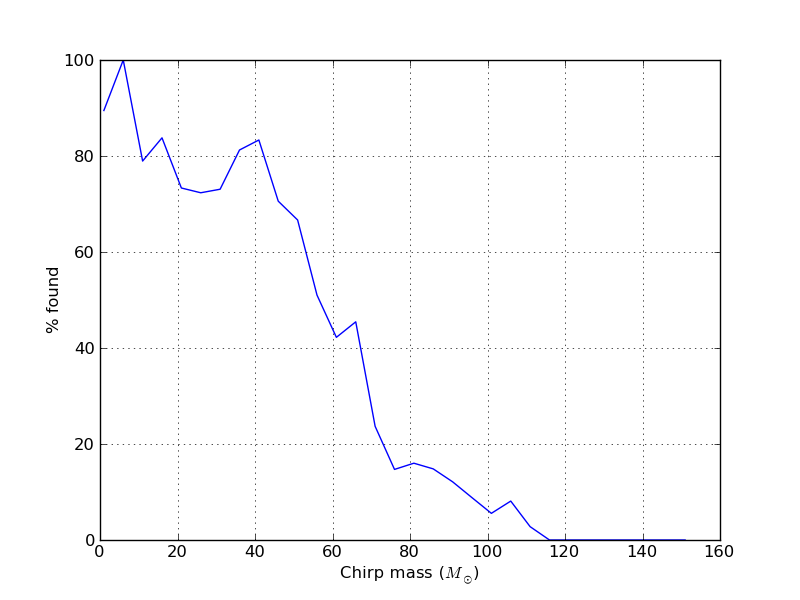
\includegraphics[width=0.5\linewidth]{figures/ninja2_results/L_second_mass_low_efficiency} \\
  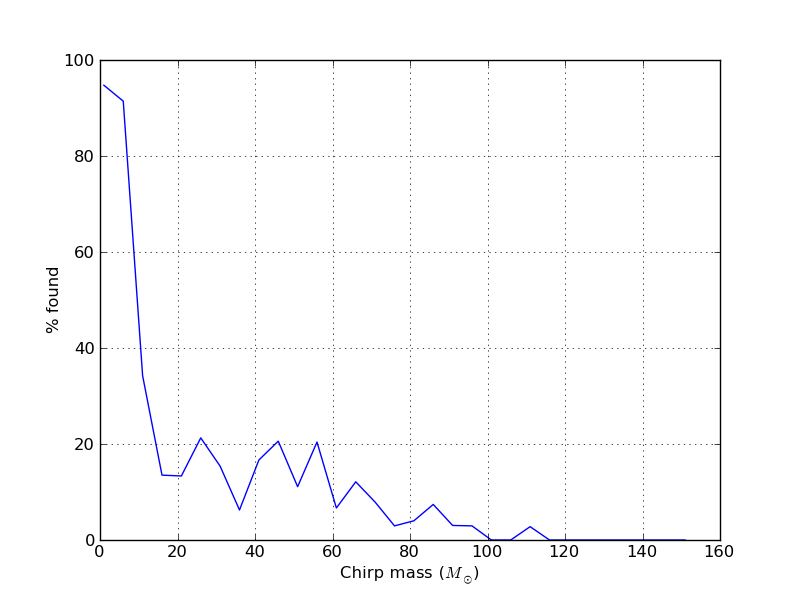
\includegraphics[width=0.5\linewidth]{figures/ninja2_results/V_second_mass_low_efficiency}
  \caption[Efficiency of the low-mass pipeline as a function of mass]{
  \label{f:low_mass_efficiencies}
Efficiencies of the low-mass pipeline as a function of mass.  As
can be seen in figure~\ref{f:ninja2_cbc_results_low_second} the
efficiencies decrease as mass increases.  However, the jaggedness in
these plots indicates that there are not enough injections to draw
definitive conclusions.
}
\end{figure}%

\begin{figure}
  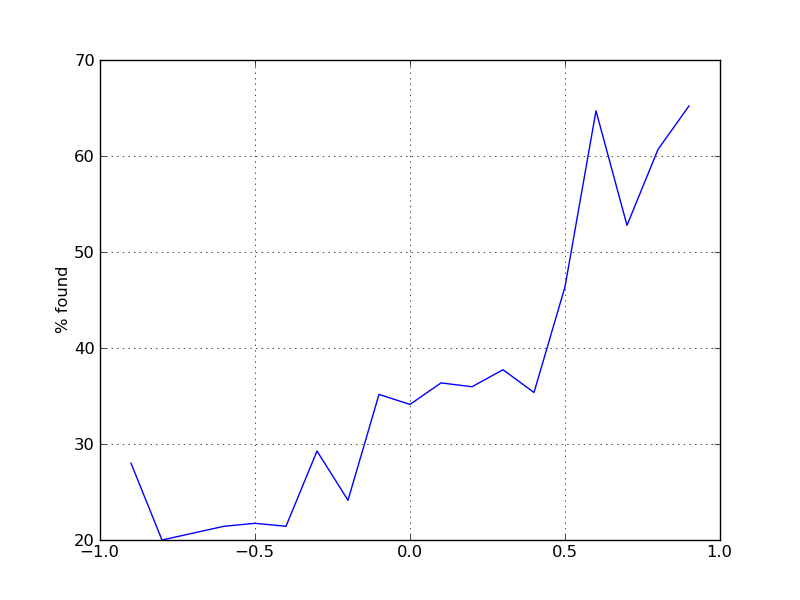
\includegraphics[width=0.5\linewidth]{figures/ninja2_results/H_second_spin_low_efficiency}
  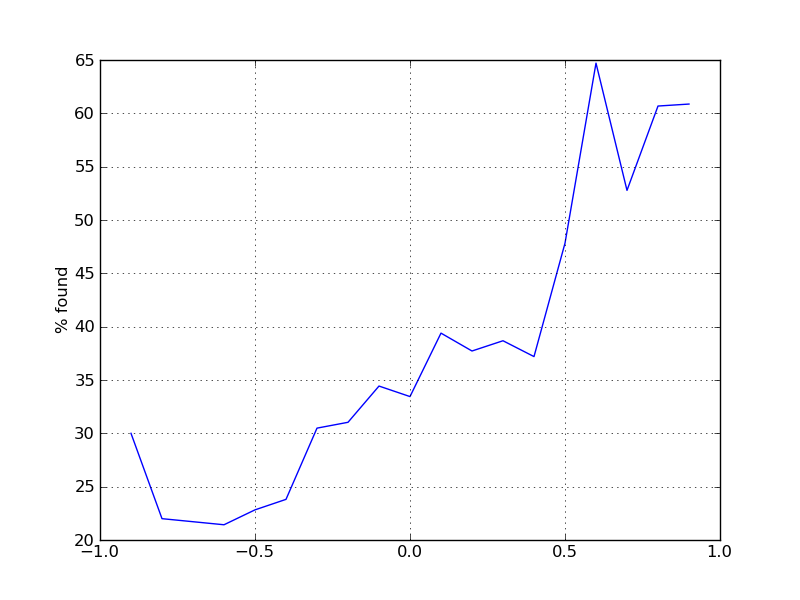
\includegraphics[width=0.5\linewidth]{figures/ninja2_results/L_second_spin_low_efficiency} \\
  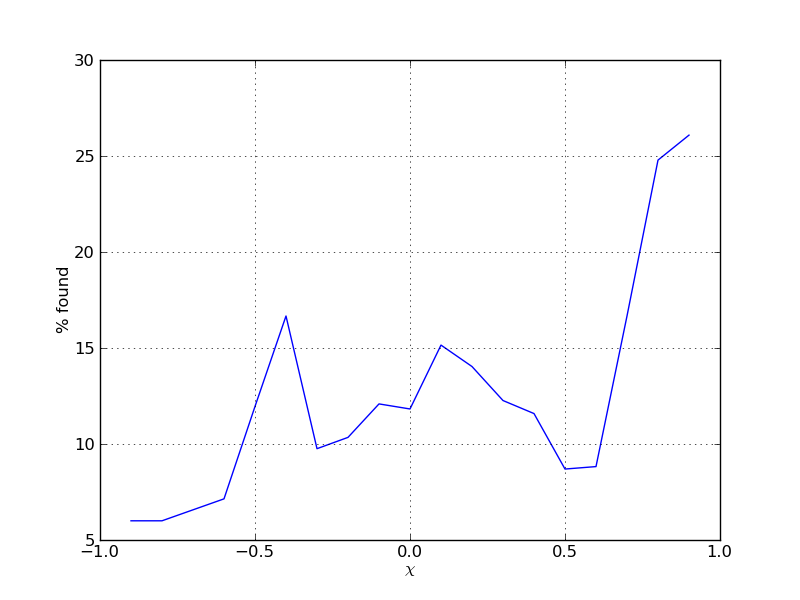
\includegraphics[width=0.5\linewidth]{figures/ninja2_results/V_second_spin_low_efficiency}
  \caption[Efficiency of the low-mass pipeline as a function of spin]{
  \label{f:low_spin_efficiencies}
Efficiencies of the low-mass pipeline as a function of the spin
parameter $\chi$.  There is a general trend suggesting the pipeline
is more efficient at detecting aligned spins, but more injections are
needed to verify and quantify this.
}
\end{figure}%


\subsection{Anomalous Virgo results}
\label{ssec:virgo_anomaly}

In both the high-mass and low-mass searches we find that at higher
chirp masses closer injections are missed while farther injections are
found.  This problem is evident in all three interferometers, but it
is most extreme in Virgo and affects even the first-stage results.  At
the time of writing no explanation for this behavior has yet been
found, however some possibilities have been ruled out.  As the problem
is most notable in Virgo we focus attention there.

First, we consider the possibility that the effective distance is
simply being misreported.  We check this by plotting the injections on
the same axes as the found/missed plots, color-coding by injected SNR.
This is shown in figure~\ref{f:anomaly_snrs}, which shows that the SNR
and effective distance, which are calculated by different portions of
the code, correlate.  This rules out this possibility.

\begin{figure}
  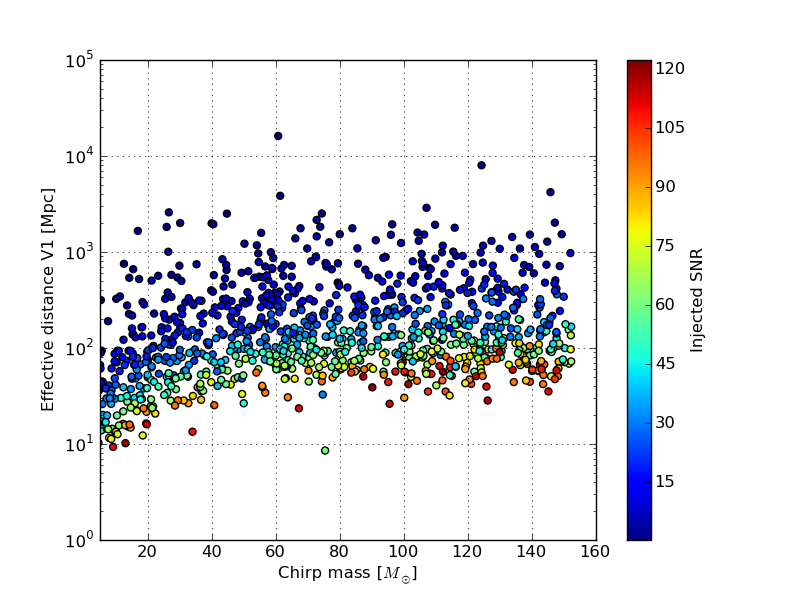
\includegraphics[width=\linewidth]{figures/ninja2_results/anomaly_snrs}
  \caption[Injections color-coded by SNR]{
  \label{f:anomaly_snrs}
Injections plotted as in the found/missed plots, color-coded by SNR.
If high SNRs corresponded to points found in Virgo it would indicate
that the effective distances were being miscalculated.  However, this
is not the case.
}
\end{figure}%

We next consider the possibility of a correlation between effective
distance and total mass.  These values are chosen randomly and
independently, but if there were some correlation such that high
effective distances corresponded to lower total masses it would
explain the results by indicating that more distant injections
happened to be more likely to fall within the range of the bank.
We again plot the injections as in the found/missed plots, now
color-coding by total mass, in figure~\ref{f:anomaly_masses}.  Again,
no correlations are seen.


\begin{figure}
  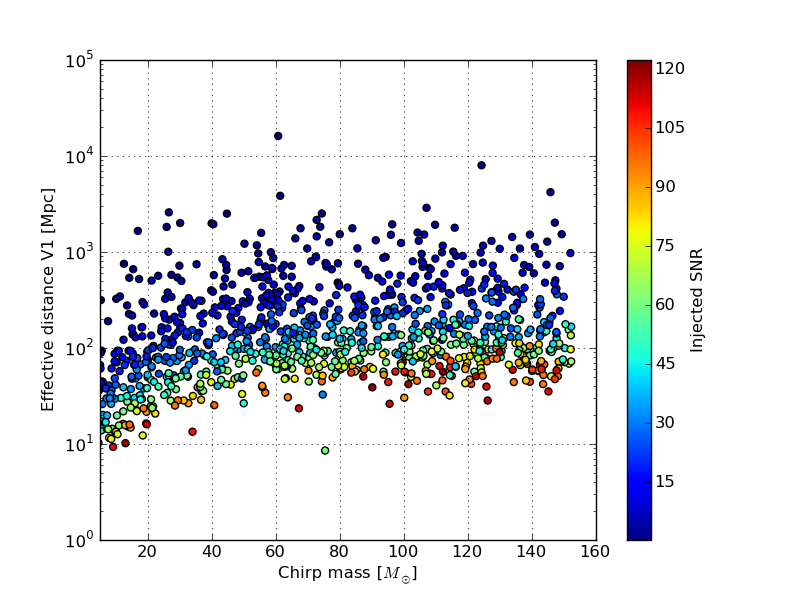
\includegraphics[width=\linewidth]{figures/ninja2_results/anomaly_snrs}
  \caption[Injections color-coded by total mass]{
  \label{f:anomaly_masses}
Injections plotted as in the found/missed plots, color-coded by total
mass.  If lower masses corresponded to points found in Virgo it would 
indicate a correlation between effective distance and mass.  However, this
is not the case.
}
\end{figure}%

Finally, we examine in detail one of the injections with chirp mass
above $100 \msun$ that is found in Virgo at the first stage beyond 100
Mpc, looking for any indication that the time series are badly
behaved.  Figure~\ref{f:anomaly_time_series} shows the injection, the
filtered data, and the SNR time series arranged so that they all cover
the same two-second interval.  All three line up as expected, at the
level of this test this injection seems to be found legitimately.

\begin{figure}
  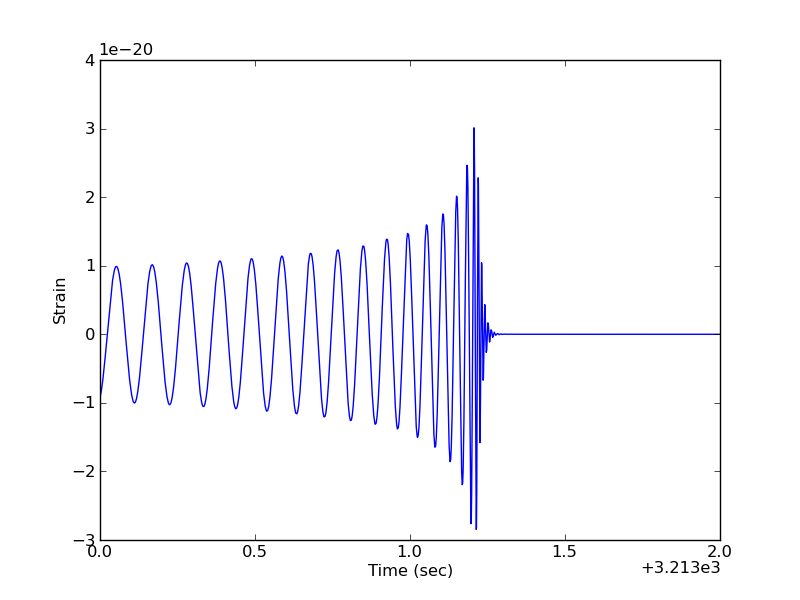
\includegraphics[width=0.5\linewidth]{figures/ninja2_results/signal}
  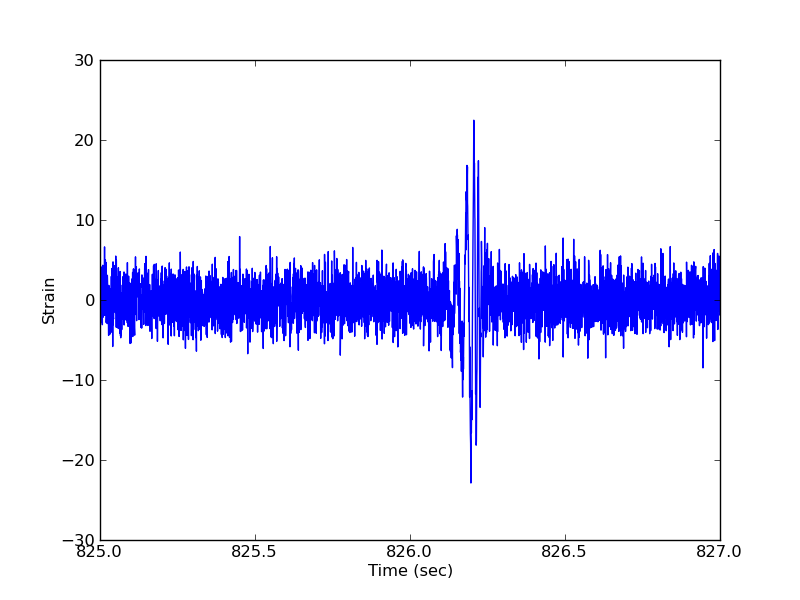
\includegraphics[width=0.5\linewidth]{figures/ninja2_results/filtered}
  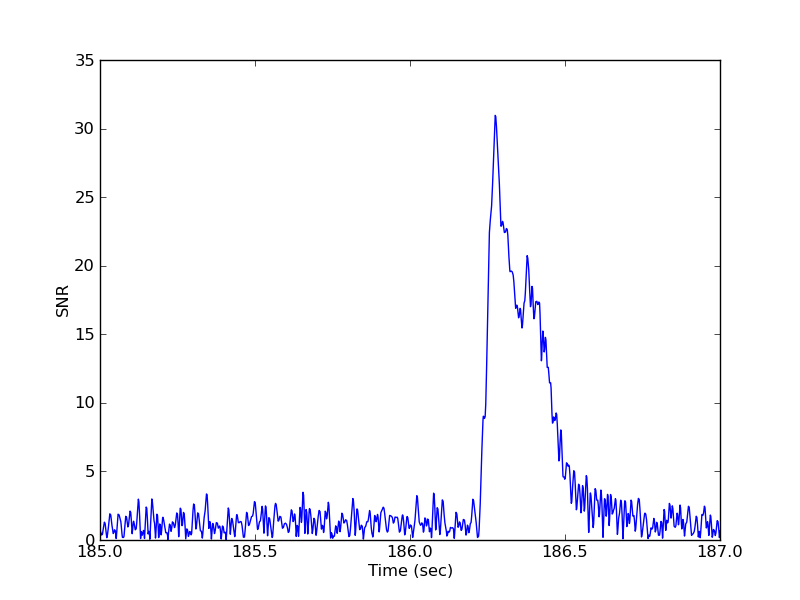
\includegraphics[width=\linewidth]{figures/ninja2_results/snr}
  \caption[Time series of an distant injection found in V1]{
  \label{f:anomaly_time_series}
Time series plots of an injection found in Virgo,  chirp mass $135
\msun$ at 157 Mpc.  Top left shows the scaled waveform.  Top right
shows the data segment passed to the matched filter,
after bandpassing to reduce low-frequency noise.  Bottom shows the SNR
time series.  All plots line up as expected.
}
\end{figure}%


\section{Open Questions for NINJA-2}

Beyond resolving the unexplained behavior in the searches we intend to
use NINJA-2 to address several important open question.  We briefly
note these here.

\weakheader{Further tests of the pipeline modifications}

We intend to rerun these analyses using a bank extended to unphysical
$\eta$ and terminating the waveforms at the WRD frequency, as in
NINJA-1.  The goal is to determine how this affects the efficiency of
the search at lower masses than could be tested in NINJA-1, as well as
on a wider range of parameter space.  We will also repeat the analysis
in real detector noise.  A critical question is how the extended bank
will affect the rate of background triggers.  NINJA-1 indicates we can
recover higher SNRs by making this change, but if this comes with an
elevated background, making signals stand out less strongly, then this
change will not be useful.

\weakheader{Transition between the low-mass and high-mass searches}

The dividing line between the low- and high-mass searches is somewhat
arbitrary at present.  We hope to use efficiency plots such as those
presented in this chapter, populated with many more injections, to
determine the point at which the efficiencies cross.  In particular,
as will be discussed in the next chapter, much of the background in
the low-mass search comes from the higher-mass end of the template
bank.  If we can reduce the upper limit of the low-mass search we can
hope to clean up the background and make quiet signals more
significant.

\weakheader{Effects of spin}

Using efficiency plots such as those presented in this chapter we hope
to determine the regions of parameter space that are not well-covered
by the existing non-spinning searches.  Such regions could then be
supplemented by spinning searches currently in development.
Conversely, by identifying regions where the current search performs
adequately we can limit the range, and hence the background, over
which spinning searches need to run.

\weakheader{Effects of template placement}

As discussed in section~\ref{sec:bank_metric}, the current searches
use a bank laid out according to a metric calculated from the Taylor
F2 stationary-phase waveform taken to 2.0 pN order in phase.  Current
searches use 3.5 pN waveforms, and the template placement is therefore
incorrect.  The extent to which it is incorrect, and the implications
for the search, can be tested by running \emph{bank simulations}.  In
such a simulation a bank is constructed and the maximum overlap
between a signal and every template in the bank is found.  By
comparing this maximum against the maximum found by varying the
parameters continuously (as in chapter~\ref{ch:comparison}) we can
determine the loss in SNR due to discretizing  the bank.  We plan to
run such analyses using the NINJA-2 signals with both 2.0 pN templates
and 3.5 pN templates in order to determine the extent to which the
incorrect metric decreases the efficiency of the search.

\section{Conclusions}

In this chapter we discussed the NINJA-2 data sets and presented
results from a one-week test run on a data set containing only low
mass signals, and a two-month set containing signals up to $350
\msun$.  The test week shows no anomalies, however when the mass range
is extended the low-mass pipeline shows unexpected behavior.  We
consider a few possibilities to explain this, but as of this writing
no explanation has been found.  It seems more likely to be a bug in
the data set generation than in the analysis, as the latter has been
much more extensively reviewed.  In either case, more study is needed.


